\documentclass[10pt,a4paper]{article}
% PACKAGES
\usepackage[utf8]{inputenc}
\usepackage[francais]{babel}
\usepackage[T1]{fontenc}

\usepackage{amsmath}
\usepackage{amsfonts}
\usepackage{amssymb}
\usepackage{hyperref}
\hypersetup{
    colorlinks=true,
    linkcolor=blue,
    filecolor=magenta,      
    urlcolor=cyan,
    pdftitle={Un document vraiment indispensable},
    pdfauthor={ED SIE !!!},
    pdfpagemode=FullScreen,
    }

\usepackage[left=2cm,right=2cm,top=2cm,bottom=2cm]{geometry}

\usepackage{lipsum}
\usepackage{booktabs}
\usepackage{lscape} % provides \landscape
\usepackage[math]{blindtext} % random text with inline math
\usepackage{multirow}
\usepackage{graphicx}

%SETUP
\title{Mon premier document \LaTeX}
\author{ED SIE}

% DOCUMENT
\begin{document}

\maketitle
\tableofcontents

\section{Introduction}
Du texte 
\subsection{Une première sous section}
Du texte 
\subsection{Une autre sous section}
Du texte 

%\lipsum % Du texte pou meubler


\section{Environnements utiles}
\label{sec:environnements}

Ceci est une liste à puces:

\begin{itemize}
	\item Une chose.
	\item Une autre chose.
\end{itemize}

Une énumération:

\begin{enumerate}
	\item Une chose.
	\item Une autre chose.
\end{enumerate}

%\lipsum % Du texte pou meubler

\section{Les maths}
Après avoir parlé des environnements dans la partie \ref{sec:environnements}. On décide maintenant de parler des mathématiques et de leur écriture dans \LaTeX. On peut écrire des équations:

$$
u_{ij}(x) = \int_0^\infty \alpha_{ij}(t,x) dt
$$

On peut aussi écrire des maths en ligne, par exemple $\alpha = 5$ est un environnement mathématique en ligne. On peut aussi numéroter les équations comme dans l'indispensable équation \ref{eq:awesome_equation} ci-dessous:

\begin{equation}
	U = \sum_{i=0}^N \dfrac{a_i}{b_i}
	\label{eq:awesome_equation}
\end{equation}

Il existe d'autres environnements de maths, par exemple:

\begin{align}
	f(x) & = (x+2)(x+4)   \\
	     & = x^2 + 6x + 8 
\end{align}

\begin{equation}
	g(x) = \left\lbrace 
	\begin{split}
		5 \mbox{ si } x \in ]-\infty, 5] \\
		0 \mbox{ otherwise }	
	\end{split}	
	\right.
\end{equation}

\section{Des tableaux avec \LaTeX}

On peut définir des tableaux avec l'environnement \og tabular \fg. 

% penser à charger \usepackage{booktabs} en haut

\begin{tabular}{lcr}
	\toprule
	\textbf{Animal} & \textbf{Classe} & \textbf{Couleur}           \\
	\midrule
	Lapin           & Mammifère      & Gris ou blanc              \\
	Truite          & Poisson         & Argentée avec des reflets \\
	\bottomrule
\end{tabular}

Il existe aussi en environnement flottant dédié aux tableaux, c'est \og table \fg. Petit exemple, la table \ref {tab:my_tab} est allée ailleurs dans le document, elle est en page \pageref{tab:my_tab}:

\blindtext[5] % random text

\begin{table}
	\begin{center}
		\begin{tabular}{lcr}
			\toprule
			\textbf{Animal} & \textbf{Classe} & \textbf{Couleur}           \\
			\midrule
			Loutre & \multirow{2}{*}{Mammifère} & Noire ? \\			
			Lapin           &  & Gris ou blanc              \\
			Truite          & Poisson         & Argentée avec des reflets \\
			\bottomrule
		\end{tabular}
		\caption{Une table définie avec l'environnement table qui la rend flottante.}
		\label{tab:my_tab}
	  \end{center}
	\end{table}
	
\blindtext[5] % random text
	
On peut aussi faire des tableaux en format paysage si ils sont trop grands horizontalement:
	
\begin{landscape}
\begin{tabular}{|c|c|c|c|c|c|c|c|c|c|c|c|}\hline

Object & Apple & Banana & Stone & Cake & Tree & Flower & House & Door & Car & Plane & Chair \\ \hline 

Quantity in Thousands & 35  &  25  & 23 & 33 & 43  & 52 & 64 & 75 & 86  & 94  & 122  \\ \hline 

\end{tabular}
\end{landscape}

Pour aller plus loin sur les tableaux, il existe des éditeurs en ligne comme \href{https://www.tablesgenerator.com/latex_tables#}{tablesgenerator}.


\section{Les figures: comment faire}

% penser à charger \usepackage{graphicx}
On peut utiliser la commande \og includegraphics \fg pour intégrer des images un peu partout:

\begin{center}
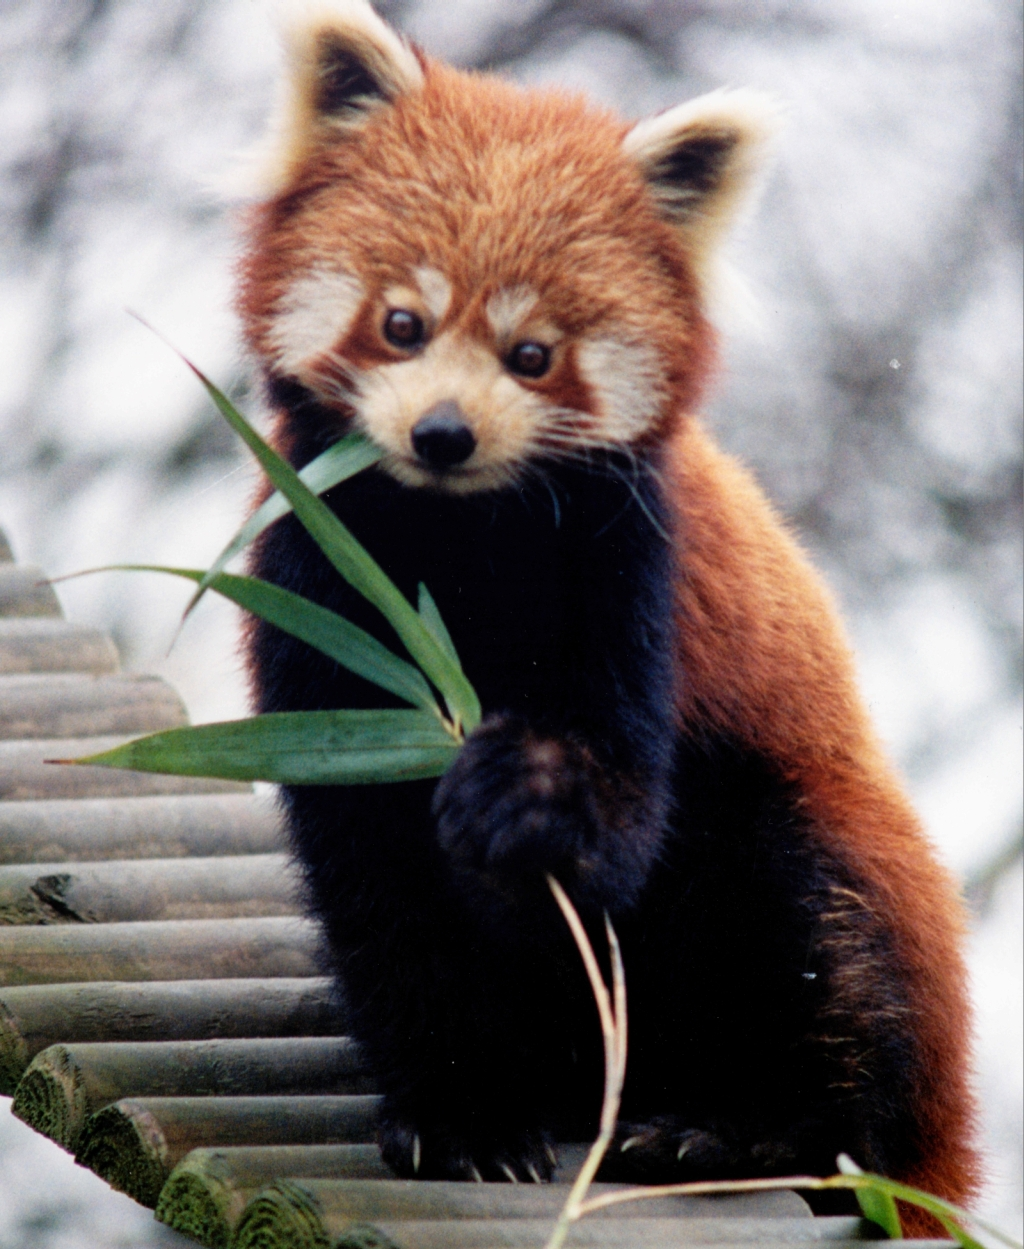
\includegraphics[width=.8\textwidth]{figures/firefox.jpg} % 80% de la largeur du texte.
\end{center}

On peut aussi le faire dans le texte 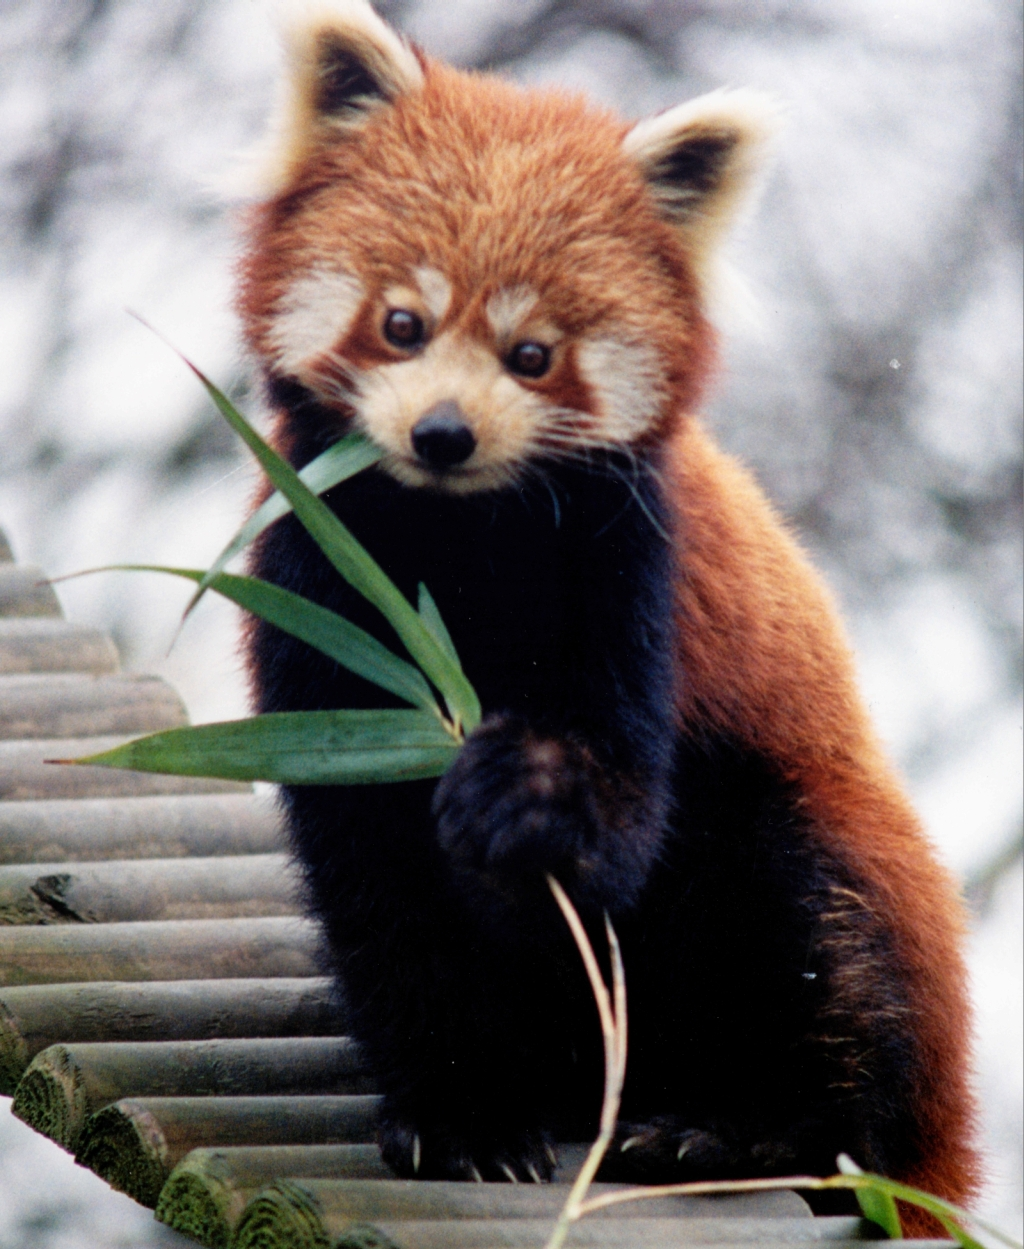
\includegraphics[width=2.5mm]{figures/firefox.jpg} et ça devrait marcher. 
Il existe une environnement flottant associé aux figures, comme le montre la figure \ref{fig:panda_roux} (p. \pageref{fig:panda_roux}).

\begin{figure}[b!]
\begin{center}
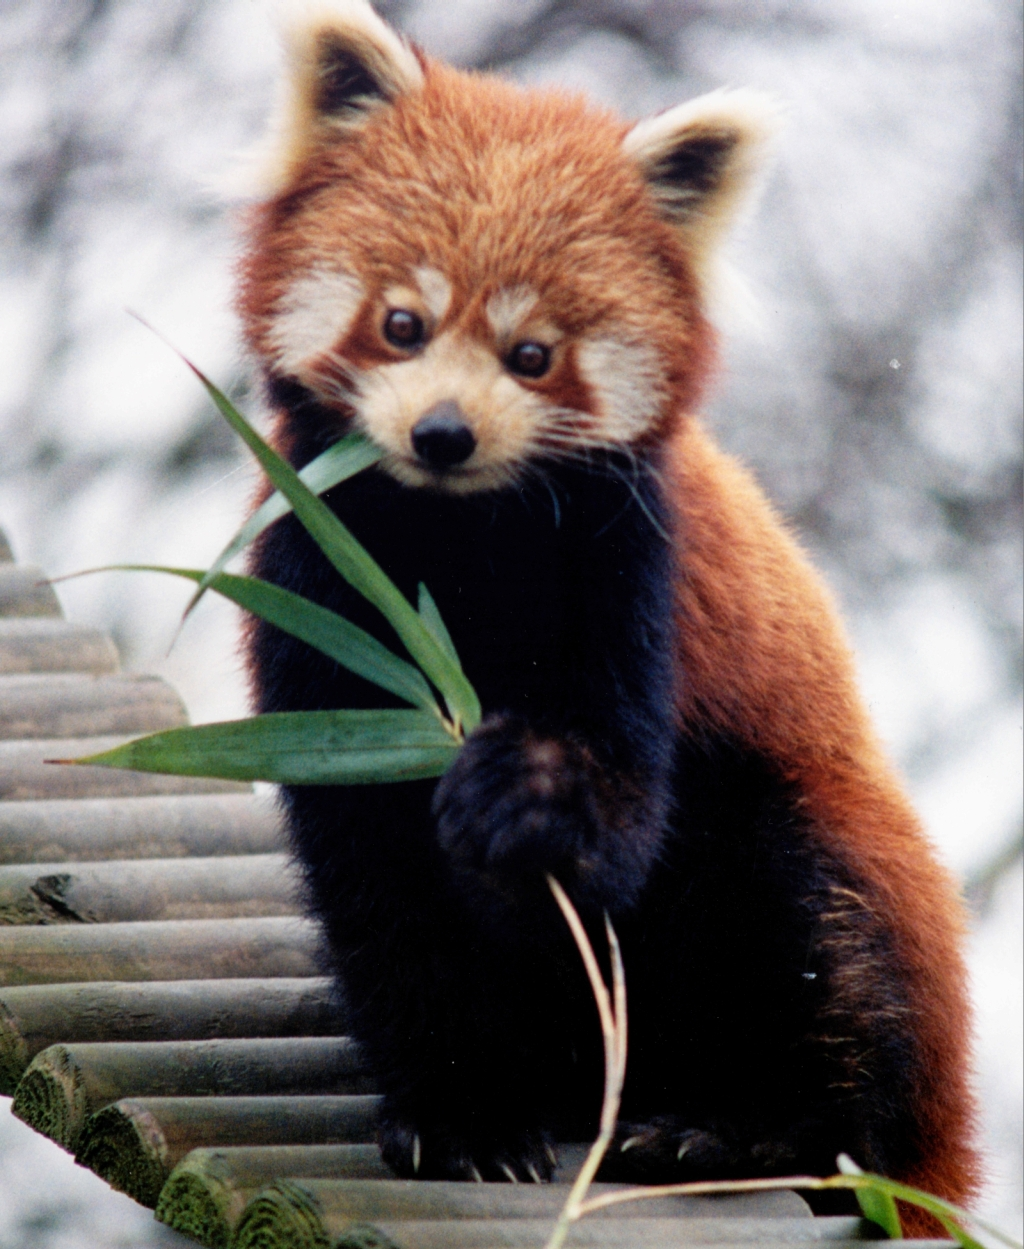
\includegraphics[width=1.\textwidth]{figures/firefox.jpg} % 80% de la largeur du texte.
\end{center}
\caption{Le Petit panda ou Panda roux (Ailurus fulgens), parfois appelé « Panda fuligineux » ou « Panda éclatant », est un mammifère protégé et en danger d'extinction de la famille des Ailuridés. 
Le panda roux est originaire de l'Himalaya et du Sud-Ouest de la Chine et préfère vivre dans les forêts montagneuses mixtes tempérées de la région, riches en bambou. }
\label{fig:panda_roux}
\end{figure}

\blindtext[10]

\blindtext[10]
	
\end{document}